\documentclass[aspectratio=169,11pt]{beamer}
\usepackage[T1]{fontenc}
\usepackage{lmodern,booktabs,tikz,amsmath}
\usetikzlibrary{arrows.meta,positioning,calc}
\definecolor{navy}{HTML}{142B45}
\definecolor{slate}{HTML}{536779}
\definecolor{gold}{HTML}{AB802E}
\setbeamercolor{normal text}{fg=navy,bg=white}
\setbeamercolor{frametitle}{fg=navy}
\setbeamercolor{structure}{fg=gold}
\setbeamerfont{frametitle}{size=\Large,series=\bfseries}
\setbeamertemplate{navigation symbols}{}
\setbeamersize{text margin left=9mm,text margin right=9mm}
\setbeamertemplate{frametitle}{\vspace{3mm}\insertframetitle\par\vspace{1mm}{\color{gold}\rule{14mm}{0.7pt}}}
\setbeamertemplate{footline}{\hspace{9mm}\scriptsize\color{slate}SCA / WORKING PAPER\hfill\insertframenumber\hspace{9mm}\vspace{3mm}}
\newcommand{\src}[1]{\par\vspace{1mm}{\fontsize{7}{8.5}\selectfont\color{slate}#1\par}}
\newcommand{\pauseq}[1]{\par\vspace{2.5mm}{\color{gold}\textbf{Pause}}\quad #1\par}
\newcommand{\bigline}[1]{{\Large #1}\par\vspace{3mm}}
\setlength{\parskip}{1.6mm}
\begin{document}
\begin{frame}{Synthetic Cultural Agents from Aggregate Anchors}
\vspace{1mm}
{\large Augusto Gonzalez-Bonorino\quad Kseniia Biriukova\quad Monica Capra}
\vspace{2mm}

{\color{slate}\small Arizona State University \quad/\quad EconLLM Lab \quad/\quad Claremont Graduate University}
\vfill
\bigline{What does an anchored synthetic policy tell us about a new survey?}
{\color{gold}Working-paper discussion\quad /\quad 16 September 2026}

\end{frame}

\begin{frame}{Before fielding an item}
\bigline{We want to learn whether proposed wording tracks a preference across populations.}
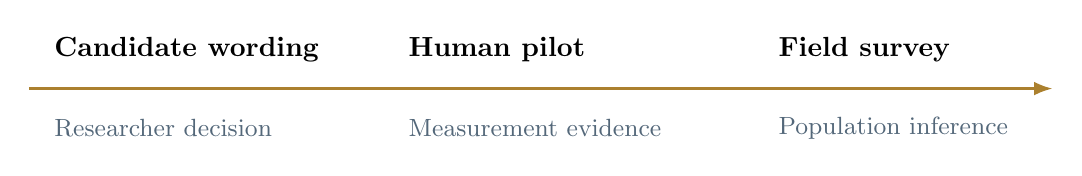
\begin{tikzpicture}[x=1cm,y=1cm]
\draw[gold,thick,-{Latex}] (0,0)--(13,0);
\foreach \x/\a/\b in {0.2/Candidate wording/Researcher decision,4.7/Human pilot/Measurement evidence,9.4/Field survey/Population inference}{\node[anchor=west,align=left] at (\x,0.5) {\textbf{\a}};\node[anchor=west,slate,font=\small] at (\x,-0.5) {\b};}
\end{tikzpicture}
\vspace{5mm}
A synthetic score could inform the first step. Its value must be tested against a subsequent human pilot.
\src{Revised paper, Introduction and Discussion. Pre-pilot usefulness is prospective.}

\end{frame}

\begin{frame}{The usual starting point is a persona prompt}
{\small\color{slate}Country-named wrapper, with the actual WVS Q57 item}
\vspace{1mm}
{\large ``Answer this questionnaire as a typical adult living in \textcolor{gold}{Argentina}.''}

``Respond naturally and sincerely, as someone would in real life. Do not mention being an AI or assistant.''

``Generally speaking, would you say that most people can be trusted or that you need to be very careful in dealing with people?''

\begin{tabular}{@{}ll}1:&Most people can be trusted\\2:&Need to be very careful\end{tabular}

{\small ``Select exactly one response code from the options below.''\\``Return only the response code, with no words or explanation.''}
\src{Appendix: evaluation wrapper; PROMPT\_SOURCE\_EXCERPTS.md: realized Q57 text. Layout reordered; chat control tokens omitted.}

\end{frame}

\begin{frame}{Make the supplied population information inspectable}
\bigline{Which information did we supply, and what can the output establish?}
\begin{columns}[T]
\begin{column}{.48\textwidth}\textbf{Declared construction input}

Aggregate preference signs determine labels on a shared comparison bank.
\end{column}
\begin{column}{.48\textwidth}\textbf{Information that remains}

Pretraining, instruction tuning, bank semantics, and fitting variation still affect scores.
\end{column}
\end{columns}
\vspace{4mm}
Country-unconditioned evaluation removes the direct country-name channel at inference.
\src{Revised paper §§1--3. Cultural fine-tuning and DPO have precedents: CultureLLM; Cao et al.; SubPOP; Jung and Kim. No broad priority claim.}

\end{frame}

\begin{frame}{The whole construction, in one view}
\vspace{-1mm}
\begin{center}
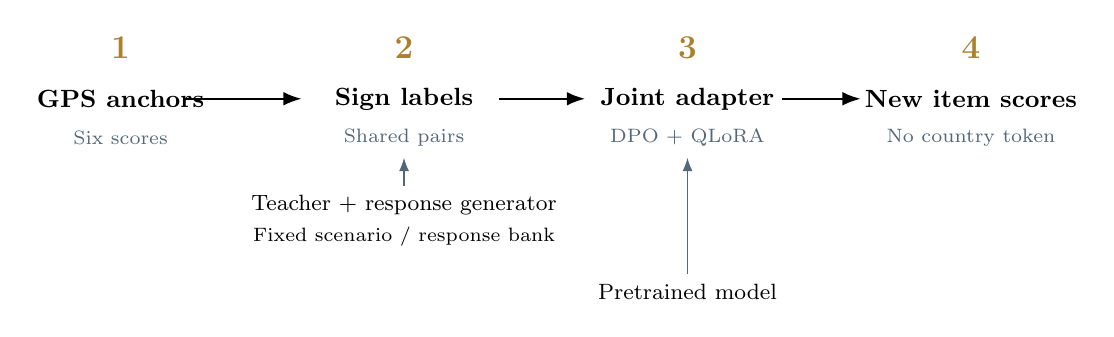
\begin{tikzpicture}[x=1cm,y=1cm,>=Latex]
\foreach \x/\n/\t/\s in {0/1/GPS anchors/Six scores,3.6/2/Sign labels/Shared pairs,7.2/3/Joint adapter/DPO + QLoRA,10.8/4/New item scores/No country token}{
\node[gold,font=\large] at (\x,1.0){\textbf{\n}};
\node[align=center,font=\bfseries\small] at (\x,.35){\t};
\node[align=center,slate,font=\scriptsize] at (\x,-.15){\s};}
\draw[thick,->] (.8,.35)--(2.3,.35);\draw[thick,->] (4.8,.35)--(5.9,.35);\draw[thick,->] (8.4,.35)--(9.4,.35);
\node[align=center,font=\footnotesize] (b) at (3.6,-1.2){Teacher + response generator\\[0.5mm]\scriptsize Fixed scenario / response bank};
\draw[->,slate] (b.north)--(3.6,-.4);
\node[align=center,font=\footnotesize] (m) at (7.2,-2.1){Pretrained model};
\draw[->,slate] (m.north)--(7.2,-.4);
\end{tikzpicture}
\end{center}
\vspace{-2mm}
\bigline{The new survey enters at readout.}
\vspace{-2mm}
\src{Custom diagram from revised paper §3 and Appendix 7. Production manifest: use\_anchors=false for optional WVS generation anchors.}

\end{frame}

\begin{frame}{Six scores become a sign profile}
\begin{center}
{\Large $z_c\quad\longrightarrow\quad s_{ck}=\mathbf{1}\{z_{ck}\geq0\}$}
\end{center}
\vspace{3mm}
\textbf{Argentina:}\quad $(-,\, +,\, -,\, +,\, +,\, -)$

{\small trust / risk / patience / altruism / pos.\ recip.\ / neg.\ recip.}

\vspace{2mm}
The United States is non-negative on all six coordinates, so every pair is labeled chosen~A. Mexico is negative on all six, so every pair is labeled chosen~B.

\vspace{2mm}
16 countries, 13 distinct sign profiles. Twins share a labeling problem: Mexico--Russia, India--Greece, Indonesia--Egypt.
\src{Revised paper §3.1 and the sign-profile table. Magnitudes and profile prose do not enter production labels.}

\end{frame}

\begin{frame}{Recipe versus invertibility}
\bigline{The map from declared signs through the bank to a policy is a construction.}
Identification would invert a named parameter from observed WVS option probabilities.

Adapter--GPS rank association on new text is criterion evidence for that construction.

Whether policies differ only as a function of the assigned sign vector remains a separate question.
\pauseq{Which of those claims should this draft make?}
\src{Revised paper §3.1. The design does not recover $z$, magnitudes, a single GPS coordinate, or culture.}

\end{frame}

\begin{frame}{A real synthetic pair receives a deterministic label}
{\color{slate}\small Positive reciprocity / bank pair \texttt{00023ac74dac}}

\textbf{Scenario, excerpt:} ``A fellow student tutored me for free before a critical exam, and now they're facing a tight deadline for their own project and need someone to review their work.''
\begin{columns}[T]
\begin{column}{.48\textwidth}\textcolor{gold}{\textbf{A / chosen for Argentina}}

``I'll set aside time to carefully review their work this evening.''
\end{column}
\begin{column}{.48\textwidth}\textbf{B / rejected for Argentina}

``I'll let them know I can only do a quick scan tomorrow morning.''
\end{column}
\end{columns}
\vspace{3mm}
$z_{c,\mathrm{positive\ reciprocity}}=+0.1596793085\quad\Rightarrow\quad A\succ B$
\src{Appendix: exact excerpts; complete pair in the Appendix. Intended trait loadings are generator judgments. The label is not an observed Argentine choice.}

\end{frame}

\begin{frame}{DPO fits the comparisons; QLoRA limits what moves}
\bigline{A regularized Bradley--Terry pairwise choice criterion}
\[
\Pr(y_w\succ y_\ell\mid x)=\sigma\!\left(\beta\left[\log\frac{\pi_\theta(y_w\mid x)}{\pi_{\rm ref}(y_w\mid x)}-\log\frac{\pi_\theta(y_\ell\mid x)}{\pi_{\rm ref}(y_\ell\mid x)}\right]\right)
\]
Increase the chosen response's relative likelihood against the rejected response, using the reference policy as the baseline.

\textbf{QLoRA:} keep the quantized Llama 3.1 8B base fixed; fit low-rank adapter weights jointly across dimensions.

\texttt{526 train / 132 held out}\qquad\texttt{rank 16 / beta 0.1 / one epoch}
\src{Revised paper §3.2 and Appendix 8; Rafailov et al.; Hu et al.; Dettmers et al. Notebook settings; checkpoint correspondence remains a release requirement.}

\end{frame}

\begin{frame}{Evaluation asks three different external questions}
\begin{columns}[T]
\begin{column}{.48\textwidth}
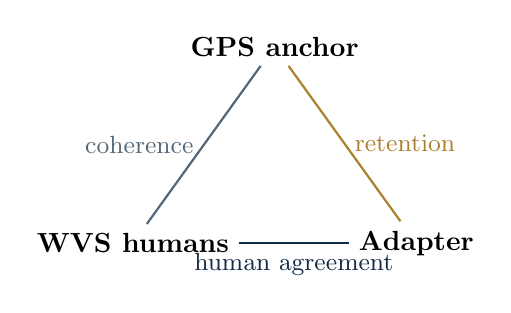
\begin{tikzpicture}[>=Latex]
\node[font=\bfseries] (g) at (0,2.5){GPS anchor};
\node[font=\bfseries] (h) at (-1.8,0){WVS humans};
\node[font=\bfseries] (a) at (1.8,0){Adapter};
\draw[slate,thick] (g)--(h) node[midway,left,font=\small]{coherence};
\draw[gold,thick] (g)--(a) node[midway,right,font=\small]{retention};
\draw[navy,thick] (h)--(a) node[midway,below,font=\small]{human agreement};
\end{tikzpicture}
\end{column}
\begin{column}{.48\textwidth}
\textbf{Same comparison surface}

16 selected countries; 23 common single-choice WVS items; same recodes and aggregation across arms.

Score supplied response codes by normalized log probabilities. No sampled answer is required.
\end{column}
\end{columns}
\vspace{4mm}
Held-out synthetic comparisons separately ask whether fitting recovers the imposed labels.
\src{Revised paper §§3.3--4. Strict common-support analysis is retrospective. Code likelihood is a scoring convention whose spread need not match population frequencies.}

\end{frame}

\begin{frame}{Fitting recovers the imposed synthetic contrasts}
\begin{columns}[T]
\begin{column}{.47\textwidth}{\Huge\color{gold}0.942}

Relative-reward recovery

{\small Chosen--rejected margin improves over the reference.}
\end{column}
\begin{column}{.47\textwidth}{\Huge\color{navy}0.819}

Raw choice accuracy

{\small Chosen response has higher adapted-model likelihood.}
\end{column}
\end{columns}
\vspace{4mm}
2,112 held-out country--pair cells reuse a shared bank. Russia has a different holdout split.
\pauseq{What independent test would make this a meaningful first-stage check?}
\src{Revised paper §4.1. Recovery is measured against synthetic labels; pooled cells are not independent human choices.}

\end{frame}

\begin{frame}{Anchor retention and human agreement differ}
\vspace{-1mm}
\begin{center}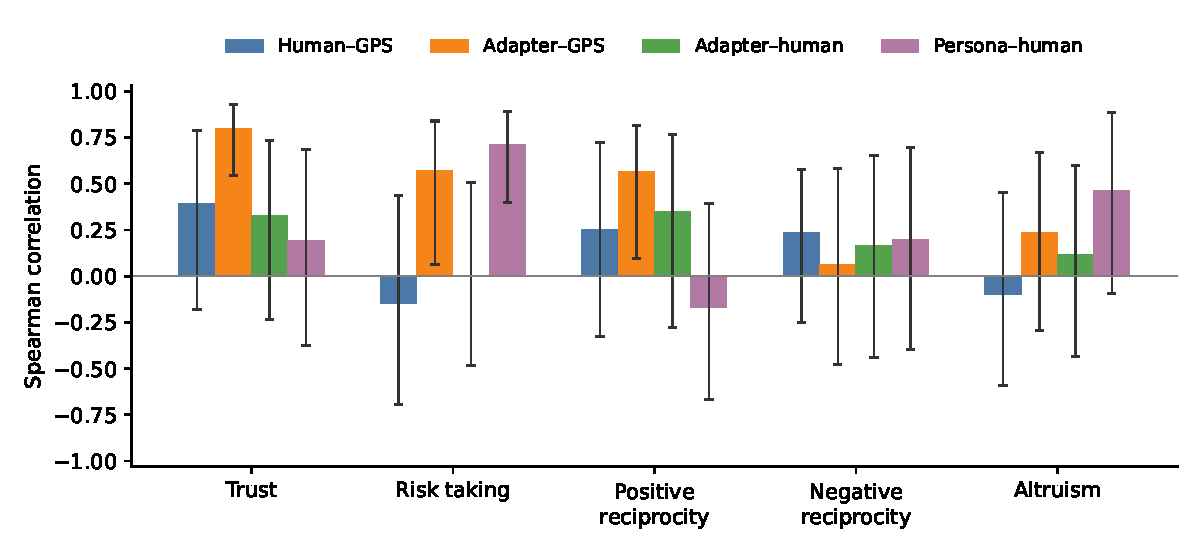
\includegraphics[width=.92\textwidth,height=4.15cm,keepaspectratio]{figures/associations.pdf}\end{center}
\vspace{1mm}
{\small Four series, different questions. Risk adapter--human has zero bar height.}
\pauseq{Which association should carry the paper's main claim?}
\src{Figure 2, unchanged. Country-bootstrap intervals; patience reported itemwise.}

\end{frame}

\begin{frame}{Trust retains the anchor; human agreement is uncertain}
\begin{center}
\begin{tabular}{@{}lrr@{}}
\toprule
Country-rank association & $\rho$ & 95\% interval\\\midrule
Adapter--GPS & \textbf{0.80} & $[0.55,\ 0.93]$\\[1.4mm]
Persona--GPS & $-0.07$ & $[-0.55,\ 0.45]$\\[1.4mm]
Adapter--human & 0.33 & $[-0.23,\ 0.74]$\\\bottomrule
\end{tabular}
\end{center}
Paired adapter-minus-persona contrast:\quad $0.87\ [0.22,1.36]$.

Permuting GPS trust $z$ across frozen adapter scores, without refitting, gives one-sided $p=0.002$.
\pauseq{Is anchor-order transfer enough for the contribution we want to make?}
\src{Revised paper §4.2 and Appendix C. Intervals omit respondent, anchor, and fitting uncertainty.}

\end{frame}

\begin{frame}{A zero does not identify the source of disagreement}
\begin{columns}[T]
\begin{column}{.46\textwidth}\textbf{Risk / adapter--human}

{\Huge\color{gold}$\rho=0$}

95\% interval $[-0.48,\ 0.51]$

Zero sample rank association establishes neither independence nor different latent constructs.
\end{column}
\begin{column}{.50\textwidth}\textbf{Patience / human--GPS}

Q43: work importance\hfill $-0.56$

Q50: financial satisfaction\hfill $+0.62$

We retain the coding and interpret these candidate indicators separately.
\end{column}
\end{columns}
\pauseq{Which independent evidence would distinguish a mapping problem from a policy limitation?}
\src{Revised paper §4.2 and Table 4. Q43 interval [-0.86,-0.04]; Q50 [0.11,0.91].}

\end{frame}

\begin{frame}{Configuration sensitivity leaves the mechanism open}
\begin{center}
\begin{tabular}{@{}lrr@{}}
\toprule
Configuration & Trust--GPS $\rho$ & Mean TVD $\downarrow$\\\midrule
Base / unconditioned & --- & 0.462\\[1mm]
Base / country persona & $-0.07$ & 0.369\\[1mm]
Adapter / unconditioned & 0.80 & 0.480\\[1mm]
Adapter / country persona & 0.67 & 0.401\\\bottomrule
\end{tabular}
\end{center}
The configuration retaining more anchor order need not resemble human response distributions more closely.

\textcolor{gold}{Next comparison:} give prompting the same anchor information.
\src{Revised paper Table 5: 23 items, 368 country--item cells. TVD is total variation distance. Base bank variation prevents interpreting a base country-ordering coefficient.}

\end{frame}

\begin{frame}{Before a journal version}
What we would run next, in that order. No new human labels.

\vspace{1mm}
{\color{gold}\textbf{1}}\quad Second scenario bank, same GPS signs, refit two adapters.

{\color{gold}\textbf{2}}\quad Sign-retrain placebo: permute signs, relabel, and refit.

{\color{gold}\textbf{3}}\quad Twin-profile check: are Mexico/Russia interchangeable on held-out WVS?

\vspace{2mm}
The assignment permutation already in the draft does not refit. Expanding 16 to 24 countries on this bank is later.
\pauseq{If we can only run one of these before submission, which one?}
\src{Paper 2 extensions. A blinded pre-pilot remains a later use-test.}

\end{frame}

\begin{frame}{What would you need to see before using this?}
\bigline{We can inspect the conditioning rule and observe trust-anchor transfer.}
Human agreement and practical pre-pilot value remain unresolved.

\par\vspace{2mm}
{\Large\color{gold}Discussion}\par\vspace{2mm}

Which part of the construction is least credible to you?

What evidence would change your view of the proposed use?

Which extension should we run first before a journal version?
\src{Working-paper claim ceiling: group-level scoring instruments intended to complement human survey research.}

\end{frame}

\begin{frame}[t]{Appendix. A complete training pair}
\footnotesize
\noindent\textbf{Scenario.} A fellow student tutored me for free before a critical exam, and now they are facing a tight deadline for their own project and need someone to review their work. Decision: I can either take the time to thoroughly review their project or concentrate on my own study schedule. Trade-off: Helping my fellow student would acknowledge the effort they put into tutoring me, but it would cut into my own study time and potentially impact my performance.

\vspace{1.2mm}
\noindent\textbf{A.} I will set aside time to carefully review their work this evening. They went out of their way to help me when it mattered most, and I want to make sure they know their effort made a difference. If I do not take this seriously, it would feel like I am ignoring the support that helped me succeed.

\vspace{1.2mm}
\noindent\textbf{B.} I will let them know I can only do a quick scan tomorrow morning. My exam prep schedule is already packed with material I have not mastered yet, and I need to be realistic about what I can manage without burning out. I hope they understand my limitations in this situation.

\normalsize
\src{Appendix 7, pair 00023ac74dac. Target: positive reciprocity. Argentina chooses A. Contractions expanded for typesetting.}

\end{frame}

\begin{frame}{Appendix. Candidate WVS indicators}
\small
\begin{center}
\begin{tabular}{@{}lp{38mm}p{62mm}@{}}\toprule
Anchor & Items & Candidate interpretation\\\midrule
Trust & Q57--Q64, Q73 & Generalized, interpersonal, institutional trust\\[1mm]
Patience & Q43; Q50 & Less work importance; financial satisfaction\\[1mm]
Risk taking & Q106, Q107, Q109, Q178 & Economic values; fare avoidance\\[1mm]
Positive reciprocity & Q81 & Confidence in charitable organizations\\[1mm]
Negative reciprocity & Q176, Q177, Q179, Q195 & Moral clarity; justifiability\\[1mm]
Altruism & Q99, Q101, Q103 & Membership in three types of organizations\\\bottomrule
\end{tabular}
\end{center}
Composites average item means without range standardization.
\src{Table 2 and Appendix 9. Strict panel excludes Q69--Q71, Q174 and Q12--Q14.}

\end{frame}

\begin{frame}{Appendix. How we score response codes}
\[
\ell_{cqj}=\sum_t\log\widehat\pi_c(a_{qjt}\mid q,a_{qj,<t}),\qquad
\widehat P_c(j\mid q)=\frac{e^{\ell_{cqj}}}{\sum_h e^{\ell_{cqh}}}
\]

Candidate strings include a leading space. Sum token log probabilities without length normalization; normalize across the supplied codes.

\[
\text{Item score}=\sum_j g_q(j)\widehat P_c(j\mid q)
\]
Human responses use the same recode before survey-weighted averaging. Item scores are then averaged within each proposed composite.
\src{Revised paper §3.3 and Appendix 7. Decoder-only model; teacher-forced scoring requires no sampled response.}

\end{frame}

\begin{frame}{Appendix. Uncertainty and remaining gates}
\textbf{Reported uncertainty}

Country bootstrap, 2,000 draws, conditional on selected countries, items, and fitted runs. Intervals omit respondent sampling, GPS measurement error, and training randomness.

\textbf{Bank and Egypt}

The shared bank is mixed-trait. Pair loadings are generator judgments. Egypt stays in the primary panel; restoring Q69--Q71 on the other fifteen countries leaves adapter--GPS trust between 0.79 and 0.81. Assignment permutation of GPS trust $z$, without refitting, gives $p=0.002$.

\textbf{Still pending}

Pinned checkpoint provenance; isolated calculation replay; independent validation of bank semantics.

\end{frame}
\end{document}
